\documentclass[../main.tex]{subfiles}
\begin{document}
  \chapter{Lecture 3}

    Recall
    \begin{displaymath}
      \ptf{\rho}{t} + \nabla \cdot (\rho \vec u) = 0,  
    \end{displaymath}
    \begin{equation}
      \quad \frac{1}{\nu} \dfrac{\nu}{t} = \nabla \cdot \vec u, 
      \quad \nu = \frac{1}{\rho},
      \label{eq:3.1}
    \end{equation}
    \begin{displaymath}
      \rho \dfrac{\vec u }{t} = \rho \left(  \ptf{\vec u}{t} + \vec u \cdot \vec u \right) = \nabla \cdot \Sigma  + \rho g,
    \end{displaymath}
    angular momentum balance
    \begin{displaymath}
      \Sigma^T = \Sigma.
    \end{displaymath}
    energy per unit mass
    \begin{equation}
      \rho \dfrac{e_0}{t} = - p (\nabla \cdot \vec u) + \Sigma' : \nabla \vec u - \nabla \cdot \vec q
      \label{eq:3.2}
    \end{equation}
    entropy per unit mass
    \begin{displaymath}
      \rho \dfrac{s}{t} = - \nabla \cdot \left( \frac{\vec q }{T} \right) + \theta,
    \end{displaymath}
    where $\theta$ is the \fndef{entopy production}. The second law of thermodynamics says that $\theta > 0 $.

    Those are complete system of balance equations and in fact quite general ones.

    \paragraph{Local thermodynamics equilibrium approximation}
    \begin{displaymath}
      \theta = \rho \dfrac{s}{t} + \nabla \cdot \left( \frac{\vec q}{T} \right),
    \end{displaymath}
    \begin{displaymath}
      s = s(e_0, \nu),
    \end{displaymath}
    and the Gibbs relation
    \begin{displaymath}
      \d s = \frac{1}{T}\d e_0 + \frac{p}{T} \d \nu.
    \end{displaymath}
    $\d e_0/\d t$ comes form the flow of a energy and the $\d \nu / \d t$ part comes from continuity equation.
    We can write it as
    \begin{displaymath}
      \rho \dfrac{s}{t} = \frac{1}{T} \underbrace{\rho \dfrac{e_0}{t}}_{\tm{Eq }\ref{eq:3.2}}
      + \frac{p}{T} \underbrace{\frac{1}{\nu} \dfrac{\nu }{t}}_{\tm{Eq } \ref{eq:3.1}},
    \end{displaymath}
    \begin{displaymath}
      \rho \dfrac{s}{t} = \frac{1}{T} \left[ - p (\nabla \cdot \vec u) + \Sigma' : \nabla \vec u - \nabla \cdot \vec q \right]
      + \frac{p}{T} (\nabla \cdot \vec u).
    \end{displaymath}
    \begin{displaymath}
      \nabla \cdot \left( \frac{\vec q }{T} \right) = \frac{1}{T} \nabla \cdot \vec q - \frac{1}{T^2} \vec q \cdot \nabla T,
    \end{displaymath}
    \begin{displaymath}
      \theta =  -\Ccancel[blue]{\frac{p}{T} (\nabla \cdot \vec u)} + \frac{1}{T} \Sigma' : \nabla \vec u -\Ccancel[red]{ \frac{1}{T} \nabla \cdot \vec q}
      + \Ccancel[blue]{\frac{p}{T} (\nabla \cdot \vec u)} + \Ccancel[red]{\frac{1}{T} \nabla \cdot \vec q} - \frac{1}{T^2} \vec q \cdot \nabla T.
    \end{displaymath}
    Thus the entropy production is given by the formula
    \begin{displaymath}
      \theta = - \frac{1}{T^2} \underbrace{\vec q \cdot \nabla T}_{\tm{heat flux}} + \frac{1}{T} \underbrace{\Sigma' : \nabla \vec u}_{\tm{momentum flux}} \geq 0.
    \end{displaymath}
    Imagine that you have a flow and a temperature gradient --- then the fluid will flow from the hotter part to the colder.
    Note that both terms have to be positive, because when one is missing, the other one must be non-negative.

    How does those equations simplify in the ideal fluid model?

    \section{Ideal fluid model}

    Recall that for the ideal fluid we have
    \begin{displaymath}
      \vec q = 0, \quad \Sigma' = 0 \qLRa \theta = 0,
    \end{displaymath}
    and therefore there is no entropy production.

    Hydrodynamics of ideal fluids:
    \begin{enumerate}
      \item $\ptf{\rho}{t} + \nabla \cdot (\rho \vec u) = 0$,
      \item $\rho \dfrac{\vec u}{t} = - \nabla p + \rho \vec g$,
      \item $ \rho \dfrac{e_0}{t} = - p(\nabla \cdot \vec u)$,
      \item $\dfrac{s}{t} = 0$.
    \end{enumerate}
    Since the 2\textsuperscript{nd} equation is a vector one we have $6$ equations. 
    Unfortunately, there are 7 unknowns, which means we are one equation short.
    The one that is missing is the thermodynamical equation of state (for pressure).

    \section{Thermodynamics}
    In the equation
    \begin{displaymath}
      e_0 = e_0(s , \nu)
    \end{displaymath}
    the specific volume as a variable is not that interesting, since it cannot be easily controlled. 
    It would be much better to use a pressure instead of $\nu$. 
    To do that we switch the thermodynamical potential, from energy to enthalpy
    \begin{displaymath}
      h_0 = e_0 + p \nu = e_0 + \frac{p}{\rho}, \quad h_0 = h_0(s, p), 
    \end{displaymath}
    \begin{displaymath}
      \d h_0 = T \d s + \nu \d p = \underbrace{T\d s}_{ = 0} + \frac{\d p}{\rho},
    \end{displaymath}
    if we work in a regime where $s$ is fixed.
    Thus 
    \begin{displaymath}
      \d h_0 = \frac{\d p}{\rho}, \quad h_0 = h_0(p),\quad \ptf{h_0}{p}|_s = \frac{1}{\rho}.
    \end{displaymath}
    Therefore $\rho = \rho(p)$ or $p = p(\rho)$ and that's what we've been missing.
    This equation is called the \fnte{equation of state}.
    
    For an ideal gas
    \begin{displaymath}
      p(\rho) = C \rho ^\gamma, \quad \gamma = \frac{c_p}{c_v}.
    \end{displaymath}

    For an ideal fluid
    \begin{displaymath}
      \rho = \rho_0 = \const.
    \end{displaymath}

    \section{Hydrostatics}
    Now that we have a complete set of equations, we can solve physical problems.
    Assume for now that $\vec u = 0$ which leads to 
    \begin{displaymath}
      \nabla p = \rho \vec g, \quad p = p(\rho).
    \end{displaymath}
    Assume that we work with an ideal gas and know the temperature profile i.e. $T(\tm{height})$.
    
    \begin{figure}[h]
      \centering
      \begin{tikzpicture}
        \draw (0,0) -- (5,0);
        \draw [-stealth] (1, 0) -- (1, 2);
        \node at (4, 1.5) {$ \vec g = - g\vez $};
        \node at (2, 1.5) {$ T(z)$ };
        \node at (0.8, 2) {$z$};
      \end{tikzpicture}
    \end{figure}

    
    \begin{displaymath}
      \dfrac{p}{z} = - \rho g, \quad p(z) = ?,
    \end{displaymath}
    For an ideal gas $p = \rho R T$, thus
    \begin{displaymath}
      \int_{p(z = )}^{p(z)} \frac{\d p'}{p'} = - \int_0^z \frac{g \d z}{RT(z)} 
      \qLRa p(z) = p(0) \exp\left( -\int_0^z \frac{g \d z}{RT(z)} \right),
    \end{displaymath}

    where we've used 
    \begin{enumerate}
      \item $T(z) \ra p(z)$
      \item $\rho(z)$ from the equation $\rho=  \frac{p}{RT}$
    \end{enumerate}

    \paragraph{Sound waves}
    Fluid in equilibrium (neglecting gravity)
    \begin{displaymath}
      \vec u = 0,
    \end{displaymath}
    and $p = p_{og} = \const.$, $\rho = \rho_{og} = \const.$, $s = s_{og} = \const.$.
    A sound wave is just a ,,small'' perturbation of the equilibrium state
    \begin{displaymath}
      \vec u ( \vec r, t) = 0 + \vec u ' (\vec r, t)  \quad (\abs{\vec u'} \ll c)
    \end{displaymath}
    \begin{displaymath}
      p ( \vec r, t) = p_{eq} + p' (\vec r, t)  \quad (p' \ll p_{eq})
    \end{displaymath}
    \begin{displaymath}
      \rho ( \vec r, t) = \rho_{eq} + \rho' (\vec r, t)  \quad (\rho ' \ll \rho_{eq}),
    \end{displaymath}
    \begin{displaymath}
      s( \vec r, t) = s_{eq} = \const.
    \end{displaymath}

    Now we want to find primed variables.
    How? By using the equations of an ideal fluid.
    We have
    \begin{equation}
      \ptf{\rho}{t} + \nabla \cdot (\rho \vec u) = 0,
    \end{equation}
    \begin{equation}
      \rho \left( \ptf{\vec u}{t} + \vec u \cdot \nabla\vec u \right) = - \nabla p,
      \label{eq:3.3}
    \end{equation}
    \begin{equation}
      s = s_{eq} = \const.
    \end{equation}

    The sound velocity squared
    \begin{displaymath}
      \nabla p = \underbrace{\left( \dfrac{p}{\rho} \right)}_{c^2}\nabla \rho = c^2 \nabla \rho.
    \end{displaymath}
    
    Those equations are very hard to solve mathematically, since they are non-linear.
    However, since we just want to solve an easier case, those can be linearly approximated.
    Omitting all second order terms, we obtain %\todo ,,og'' should be changed to ,,eq'' XD.
    \begin{displaymath}
      \ptf{(\rho_{eq} + \rho')}{t} + \nabla \cdot \left[ (\rho_{eq} + \rho') \vec u \right] = 0,
    \end{displaymath}
    and the \fnte{linearized continuity equation}
    \begin{equation}
      \nabla \cdot \vec u' = - \frac{1}{\rho_{eq}} \ptf{\rho'}{t}.
      \label{eq:lincont}
    \end{equation}

    Now we take care of the second equation (\ref{eq:3.3})
    \begin{displaymath}
      (\rho_{eq} + \rho') \left[ \ptf{\vec u'}{t} + \underbrace{\vec u' \cdot \nabla \vec u'}_{\approx 0} \right] = - c^2 \nabla (\rho_{eq} + \rho'),
    \end{displaymath}
    and obtain the \fnte{linearized equation of motion}
    \begin{displaymath}
      \ptf{\vec u'}{t} = - \frac{c^2}{\rho_{eq}} \nabla \rho'.
    \end{displaymath}

    We have the following system
    \begin{align*}
      \nabla \cdot \vec u' = - \frac{1}{\rho_{eq}} \ptf{\rho'}{t}, \\
      \ptf{\vec u'}{t} = - \frac{c^2}{\rho_{eq}} \nabla \rho'.
    \end{align*}
    Differentiating the first equation with respect to time and using divergence operator on the second one we get
    \begin{displaymath}
      \dptf{(\rho')}{t} = c^2 \nabla^2 \rho'.
    \end{displaymath}

    So the speed of sound
    \begin{displaymath}
      c^2 = \left( \ptf{p}{\rho} \right)_s.
    \end{displaymath}
    For $s = \const$, $p(\rho) = C \rho^\gamma$, it can be approximated as
    \begin{displaymath}
      \left( \ptf{p}{\rho} \right)_s = \gamma \frac{p}{\rho} \approx \gamma\frac{p_{eq}}{\rho_{eq}}.
    \end{displaymath}
    \begin{displaymath}
      c^2 \approx \gamma \frac{p_{eq}}{\rho_{eq}} = \gamma R T_{eq}.
    \end{displaymath}
    

    \paragraph{1-D wave equation}
    \begin{equation}
      \dptf{(\rho')}{t} = c^2 \dptf{(\rho')}{x}, \quad \rho'(x, t) = ?.
      \label{eq:1Dwave}
    \end{equation}
    To solve it we write $\rho'$ in a Fourier representation
    \begin{displaymath}
      \rho'(x,t) = \int\d k \int \d \omega \rho'(k, \omega) e^{ik x} e^{-i\omega t}.
    \end{displaymath}
    Substituting the above into \ref{eq:1Dwave} we get
    \begin{displaymath}
      (- i \omega) ^2 \rho'(k, \omega) = c^2 (i k)^2 \rho'(k,\omega),
    \end{displaymath}
    \begin{displaymath}
      \omega^2 = c^2 k^2 \qLRa \omega = \pm c k.
    \end{displaymath}
    The above equation is called the \fndef{dispersion relation}.
    Using it we get
    \begin{displaymath}
      \exp\left[ i (k x - \omega t) \right] = \exp\left[ i k (x - c t)\right].
    \end{displaymath}

    Finally
    \begin{displaymath}
      \rho'(x, t) = \int \d k \rho_1'(x) \exp\left( i k (x - c t) \right) + \int \d k \rho_2' \exp(ik ( x + ct)),
    \end{displaymath}
    which are two families of perturbations travelling in the opposite directions.

    \paragraph{3D case}

    Using Fourier representation
    \begin{displaymath}
      \rho'(\vec r, t) = \int \d \vec k \int \d \omega \rho'(\vec k, \omega) \exp\left[ i( \vec k \cdot \vec r - \omega t )\right],
    \end{displaymath}
    \begin{displaymath}
      \dptf{(\rho')}{t} = c^2 \nabla^2 \rho',
    \end{displaymath}
    \begin{displaymath}
      (- i\omega)^2 \rho'(\vec k, \omega) - c^2 (i\vec k)^2 \rho'(\vec k, \omega) \qLRa \omega = \pm c \abs{k},
    \end{displaymath}
    \begin{displaymath}
      \exp\left[ i(\vec k \cdot \vec r - \omega t) \right] = \exp\left[ i k ( \hat{k} \cdot \vec r - c t \right].
    \end{displaymath}
    Note that $c$ doesn't depend on $\omega$. 
    If it would, we will call such wave \fndef{dispersive}.
    Nondispersive waves travel without changing shape.

    We know $\rho'(\vec r, t)$. What about $p'(\vec r, t)$ and $\vec u'(\vec r, t)$?

    By substituting into
    \begin{displaymath}
      \d p = \left( \frac{p}{\rho} \right)_s \d \rho, 
    \end{displaymath}
    relations $p'(\vec r, t) = c^2 \rho'(\vec r, t)$, we can calculate $p'(\vec r, t)$.

    To obtain velocity $\vec u$ we note that
    \begin{displaymath}
      \ptf{\vec u'}{t}  = - \frac{c^2}{\rho_{eq}} \nabla \rho'
    \end{displaymath}
    and, by using Fourier transform, we obtain
    \begin{displaymath}
      \vec u' (\vec k, \omega) = \frac{c^2}{\rho_{eq}\omega}\vec k \rho'(\vec k, \omega) 
      = \pm\frac{c^2}{\rho_{eq} ck } \vec k \rho'(\vec k, \omega) 
    \end{displaymath}
    \begin{displaymath}
      \vec u' = \pm  \frac{c}{\rho_{eq}} \rho' \hat k.
    \end{displaymath}
    Sound waves are longitudinal (particles move in the same way the waves propagates).

    \section{Aerodynamics}

    Imagine that there is a wing profile and consider a wind tunel configuration.

    \begin{figure}[h]
      \centering
      \begin{tikzpicture}
        \node[anchor=south west] (image) at (0,0)
        {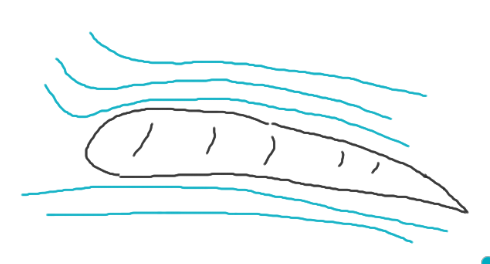
\includegraphics[width=0.25\textwidth]{./images/02Fig1.png}};
          \begin{scope}[x={(image.south east)}, y={(image.north west)}]
          % \node at (0.0, 0.0) {};
          \draw [-stealth] (0.5, 0.45) -- (0.6, 0.85);
          \draw [dashed, red, -stealth] (0.5, 0.45) -- (0.5, 0.85);
          \draw [dashed, green, -stealth] (0.5, 0.45) -- (0.6, 0.45);
          \node at (0.4, 0.8) {lift};
          \node at (0.6, 0.3) {drag};
          \end{scope}
      \end{tikzpicture}
      \label{fig:}
    \end{figure}

    Question: what is the force that the flow exerts on the object?
    The force can be decomposed into two parts: the lift and the drag.
    \begin{displaymath}
      \vec F = -\int_S p \hat{n} \d s, \quad p(\vec r, t) = ?
    \end{displaymath}

    To obtain $p$, $\vec u$ and $\vec F$ we have to solve Euler's equations
    \begin{align*}
      \rho\left( \ptf{\vec u}{t} + \vec u \cdot \nabla \vec u \right) = - \nabla p + \rho \vec g\\
      \ptf{p}{t} + \rho \cdot (\rho \vec u) = 0.
    \end{align*}
    Those are most often almost impossible to solve.
    We should try to simplify the mathematical problem here.

    First we can try choosing a different variable.
    We change $\vec u$ into \fndef{vorticity} $\vec \xi = \nabla \times \vec u$.
    
    \begin{figure}
      \centering
      \begin{tikzpicture}
        \node[anchor=south west] (image) at (0,0)
        {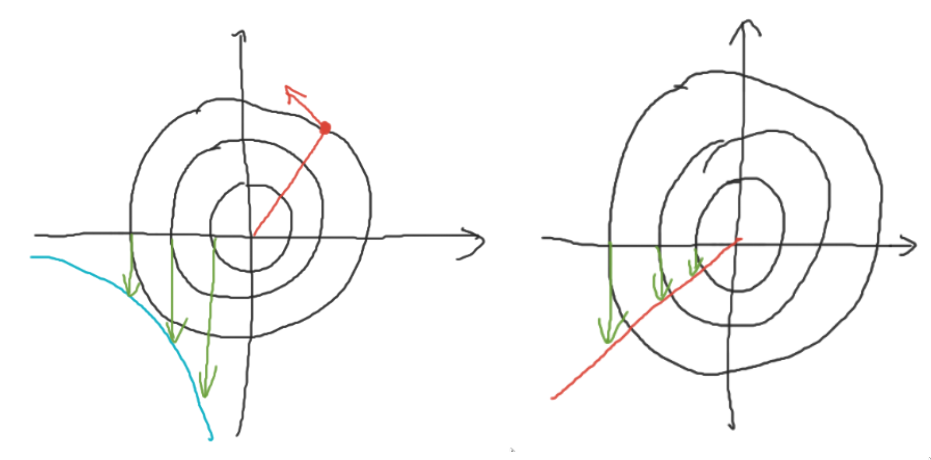
\includegraphics[width=0.65\textwidth]{./images/02Fig2.png}};
          \begin{scope}[x={(image.south east)}, y={(image.north west)}]
          \node at (0.0, 0.0) {};
          \end{scope}
      \end{tikzpicture}
      \label{fig:}
    \end{figure}

    Euler's equations
    \begin{displaymath}
      \ptf{\vec u}{t}+ \vec u \cdot \nabla \cdot \vec u= - \frac{1}{\rho} \nabla p + \vec g
    \end{displaymath}
    \begin{enumerate}
      \item $ \vec g = - \nabla \chi$
      \item 
        \begin{displaymath}
          \vec u \cdot \nabla \cdot \vec u = \nabla \left( \frac{\vec u^2}{2} \right) + (\nabla \times \vec u) \times \vec u 
          = \nabla \left( \frac{\vec u^2}{2} \right) + \vec \xi \times \vec u
        \end{displaymath}
      \item $ \frac{1}{\rho} \nabla p = \nabla h_0$
    \end{enumerate}
    \begin{equation}
      \ptf{\vec u}{t} + \nabla \times \vec u = - \nabla h_0 - \nabla \left( \frac{\vec u^2}{2} \right) - \nabla \chi
      = - \nabla \left( h_0 + \frac{1}{2} \vec u^2 \chi \right) =: - \nabla  \mathfrak{h},
      \label{eq:3.4}
    \end{equation}
    where
    \begin{displaymath}
      \mathfrak{h} = h_0 + \frac{ \vec u^2}{2} + \chi .
    \end{displaymath}

    Then Equation \ref{eq:3.4} reads
    \begin{displaymath}
      \ptf{\vec u}{t} + \vec \xi \times \vec u = - \nabla \mf{h}.
    \end{displaymath}
    By taking the rotation of both sides 
    \begin{displaymath}
      \ptf{\overbrace{\nabla \times \vec u}^{\xi}}{t} + \nabla \times (\vec \xi \times \vec u) = 0,
    \end{displaymath}

    we obtain
    \begin{displaymath}
      \nabla \times (\vec \xi \times \vec u) = ( \vec u \cdot \nabla) \vec \xi - (\vec \xi \cdot \nabla) \vec u 
      + \xi (\nabla \cdot \vec u) - \vec u (\nabla \cdot \vec \xi)=
    \end{displaymath}
    if the flow is incompressible
    \begin{displaymath}
      \ptf{\vec \xi}{t} + \vec u \cdot \nabla \vec \xi = \vec \xi \cdot \nabla \cdot \vec u
    \end{displaymath}
    \begin{displaymath}
      \dfrac{\vec \xi}{t} = \vec \xi \cdot \nabla \vec \xi.
    \end{displaymath}

    If $\nabla \vec u = 0$ the $\xi $ is an invariant of a motion.
\end{document}
